%====================================================================
%====================================================================
\section{Extensions of block-models}
%====================================================================
\subsection{Covariates}
\frame{\frametitle{Outline} \tableofcontents[currentsection]}
%====================================================================
\frame{\frametitle{Accounting for covariates} 

  \paragraph{Adding a regression term.}
  \begin{itemize}
  \item Information about similarity or dissimilarity between species is often available \\
  \ra taxonomic, phylogenetic or geographic distance
  \item \bigskip Obvious generalization of the stochastic block-model \refer{MRV10}:
  $$
  Y_{ij} \sim \Pcal(\exp(\alpha_{Z_iZ_j} + x_{ij}^\intercal \beta))
  $$
  \ra $x_{ij} =$ vector of covariates for the pair $(i, j)$
  \item \bigskip Parameters: $\theta = (\pi, \alpha, \beta)$
  \end{itemize}

  \pause \bigskip \bigskip 
  \paragraph{Variational EM algorithm.} \refer{MRV10}
  \begin{itemize}
  \item Very similar to SBM without covariates
  \item \bigskip Estimation of $\beta$ via weighted generalized linear model
  \end{itemize}

}

%====================================================================
\frame{\frametitle{Tree species network} 

  \begin{tabular}{ccc}
    \hspace{-.04\textwidth}
    \begin{tabular}{p{.35\textwidth}}
      \paragraph{Covariate:}
      $$
      x_{ij} = \text{taxonomic distance}
      $$
      ~ \\

      \paragraph{Estimates:}
      $$
      \widehat{K}_{ICL} = 4
      $$
      $$
      \widehat{\beta} = -.317
      $$
      \onslide+<2->{\begin{itemize}
      \item Taxonomy (partially) explains the links (smaller $\widehat{K}$)
      \item \bigskip Distant species share less parasites ($\widehat{\beta} < 0$)
      \item \bigskip The remaining structure is \emphase{not related to taxonomy}
      \end{itemize}}
    \end{tabular}
    &
    \hspace{-.05\textwidth}
    \begin{tabular}{p{.3\textwidth}}
      \paragraph{No covariate:} $\widehat{K}_{ICL} = 7$ \\
      \includegraphics[height=.3\textwidth, width=.3\textwidth]{\fignet/Tree-adjMat-SBMnull} \\
      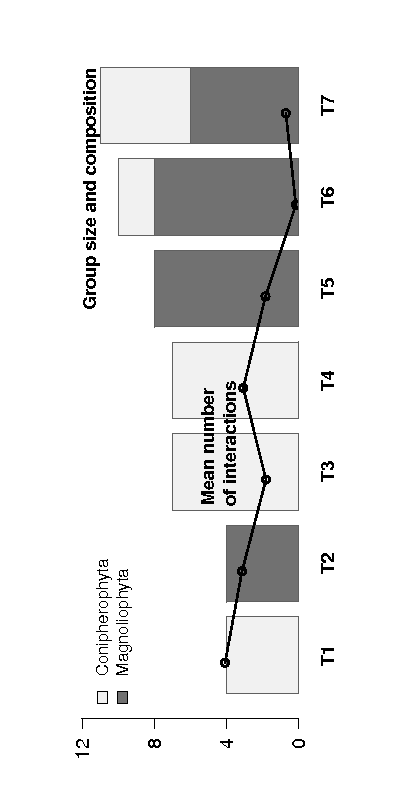
\includegraphics[height=.3\textwidth, width=.3\textwidth, trim=150 150 150 150]{\fignet/MRV10_AoAS_Q7_group}
    \end{tabular}
    &
    \hspace{-.05\textwidth}
    \begin{tabular}{p{.3\textwidth}}
      \paragraph{Taxonomic dist.:} $\widehat{K}_{ICL} = 4$ \\
      \includegraphics[height=.3\textwidth, width=.3\textwidth]{\fignet/Tree-adjMat-SBMtaxo} \\
      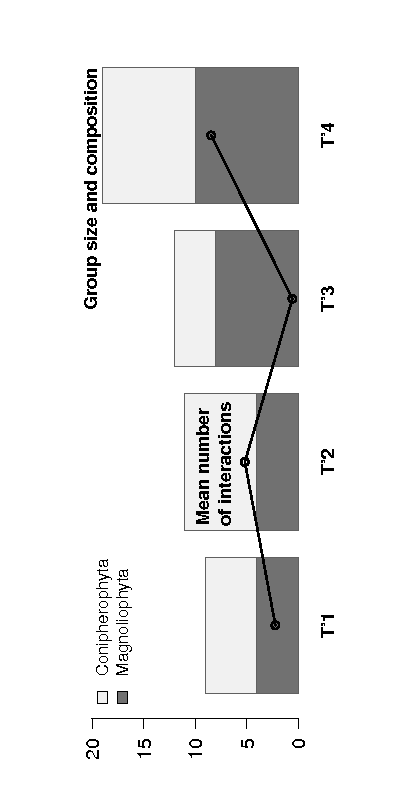
\includegraphics[height=.3\textwidth, width=.3\textwidth, trim=150 150 150 150]{\fignet/MRV10_AoAS_Q4_group}
    \end{tabular}
  \end{tabular}

}

%====================================================================
\subsection{Dynamic SBM}
%====================================================================
\frame{\frametitle{Animal behavior} 

  \paragraph{Data:} \refer{RSF15}
  \begin{itemize}
   \item Consider $n$ individuals (animals) along $T$ times (days, weeks)
   \item \bigskip At each time, observe
   $$
   Y_{ij}^t = \text{intensity of the social interaction between individuals $i$ and $j$ at time $t$}
   $$
  \end{itemize}
  
  \bigskip \bigskip \pause
  \paragraph{Questions:} 
  \begin{itemize}
  \item Do the individuals play different roles in the social network 
  \item \bigskip Do these roles change over time
  \end{itemize}

}

%====================================================================
\frame{\frametitle{Dynamic SBM} 

  \paragraph{Dynamic stochastic block-model.}   \refer{MaM17}
  \begin{itemize}
  \item Assume that individuals belong to $K$ clusters ('roles')
  \item \bigskip Denote by $Z_i^t$ the (latent) role of individual $i$ at time $t$
  \item \bigskip The successive roles of each individuals are independent Markov chains
  $$
  Z_i = \{Z_i^t\}_{1 \leq t \leq T} \sim MC(\nu_1, \pi)
  $$
  \item Social interactions are conditionally independent
  $$
  \{Y_{ij}^t\}_{i, j, t} \text{independent } \mid \{Z_i^t\}_{i, t}, \qquad
  Y_{ij}^t \mid Z_i^t, Z_j^t \sim F(\cdot; \gamma_{Z_i^t, Z_j^t})
  $$
  \end{itemize}  
  $$
  \begin{overprint}
    \onslide<2>  \begin{tikzpicture}
    \node[nocircle] (LL) at (-0.5*\edgeunit,-0.5*\edgeunit) {};
  \node[nocircle] (UL) at (-0.5*\edgeunit, 2.5*\edgeunit) {};
  \node[nocircle] (UR) at ( 5.0*\edgeunit, 2.5*\edgeunit) {};
  \node[nocircle] (UL) at ( 5.0*\edgeunit,-0.5*\edgeunit) {};

  \node[hidden] (Z11) at (0.0*\edgeunit,  2.0*\edgeunit) {$Z^1_1$};
  \node[hidden] (Z21) at (0.0*\edgeunit,  1.0*\edgeunit) {$Z^1_i$};
  \node[hidden] (Z31) at (0.0*\edgeunit,  0.0*\edgeunit) {$Z^1_n$};

  
\end{tikzpicture}

    \onslide<3>  \begin{tikzpicture}
    \node[nocircle] (LL) at (-0.5*\edgeunit,-0.5*\edgeunit) {};
  \node[nocircle] (UL) at (-0.5*\edgeunit, 2.5*\edgeunit) {};
  \node[nocircle] (UR) at ( 5.0*\edgeunit, 2.5*\edgeunit) {};
  \node[nocircle] (UL) at ( 5.0*\edgeunit,-0.5*\edgeunit) {};

  \node[hidden] (Z11) at (0.0*\edgeunit,  2.0*\edgeunit) {$Z^1_1$};
  \node[hidden] (Z21) at (0.0*\edgeunit,  1.0*\edgeunit) {$Z^1_i$};
  \node[hidden] (Z31) at (0.0*\edgeunit,  0.0*\edgeunit) {$Z^1_n$};

  \node[observed] (Y121) at (1.0*\edgeunit, 1.8*\edgeunit) {$Y^1_{1i}$};
  \node[observed] (Y131) at (1.0*\edgeunit, 1.0*\edgeunit) {$Y^1_{1n}$};
  \node[observed] (Y231) at (1.0*\edgeunit, 0.2*\edgeunit) {$Y^1_{in}$};
  

  
  \draw[arrow] (Z11) to (Y121);  \draw[arrow] (Z11) to (Y131);  
  \draw[arrow] (Z21) to (Y121);  \draw[arrow] (Z21) to (Y231);  
  \draw[arrow] (Z31) to (Y131);  \draw[arrow] (Z31) to (Y231);  
  
\end{tikzpicture}

    \onslide<4>  \begin{tikzpicture}
    \node[nocircle] (LL) at (-0.5*\edgeunit,-0.5*\edgeunit) {};
  \node[nocircle] (UL) at (-0.5*\edgeunit, 2.5*\edgeunit) {};
  \node[nocircle] (UR) at ( 5.0*\edgeunit, 2.5*\edgeunit) {};
  \node[nocircle] (UL) at ( 5.0*\edgeunit,-0.5*\edgeunit) {};

  \node[hidden] (Z11) at (0.0*\edgeunit,  2.0*\edgeunit) {$Z^1_1$};
  \node[hidden] (Z21) at (0.0*\edgeunit,  1.0*\edgeunit) {$Z^1_i$};
  \node[hidden] (Z31) at (0.0*\edgeunit,  0.0*\edgeunit) {$Z^1_n$};

  \node[hidden] (Z12) at (2.0*\edgeunit,  2.0*\edgeunit) {$Z^2_1$};
  \node[hidden] (Z22) at (2.0*\edgeunit,  1.0*\edgeunit) {$Z^2_i$};
  \node[hidden] (Z32) at (2.0*\edgeunit,  0.0*\edgeunit) {$Z^2_n$};

  \node[observed] (Y121) at (1.0*\edgeunit, 1.8*\edgeunit) {$Y^1_{1i}$};
  \node[observed] (Y131) at (1.0*\edgeunit, 1.0*\edgeunit) {$Y^1_{1n}$};
  \node[observed] (Y231) at (1.0*\edgeunit, 0.2*\edgeunit) {$Y^1_{in}$};
  

  
  \draw[arrow] (Z11) to (Y121);  \draw[arrow] (Z11) to (Y131);  
  \draw[arrow] (Z21) to (Y121);  \draw[arrow] (Z21) to (Y231);  
  \draw[arrow] (Z31) to (Y131);  \draw[arrow] (Z31) to (Y231);  
  
  \draw[arrowbendleft] (Z11) to (Z12);  
  \draw[arrowbendleft] (Z21) to (Z22);  
  \draw[arrowbendright] (Z31) to (Z32);
  
\end{tikzpicture}

    \onslide<5>  \begin{tikzpicture}
    \node[nocircle] (LL) at (-0.5*\edgeunit,-0.5*\edgeunit) {};
  \node[nocircle] (UL) at (-0.5*\edgeunit, 2.5*\edgeunit) {};
  \node[nocircle] (UR) at ( 5.0*\edgeunit, 2.5*\edgeunit) {};
  \node[nocircle] (UL) at ( 5.0*\edgeunit,-0.5*\edgeunit) {};

  \node[hidden] (Z11) at (0.0*\edgeunit,  2.0*\edgeunit) {$Z^1_1$};
  \node[hidden] (Z21) at (0.0*\edgeunit,  1.0*\edgeunit) {$Z^1_i$};
  \node[hidden] (Z31) at (0.0*\edgeunit,  0.0*\edgeunit) {$Z^1_n$};

  \node[hidden] (Z12) at (2.0*\edgeunit,  2.0*\edgeunit) {$Z^2_1$};
  \node[hidden] (Z22) at (2.0*\edgeunit,  1.0*\edgeunit) {$Z^2_i$};
  \node[hidden] (Z32) at (2.0*\edgeunit,  0.0*\edgeunit) {$Z^2_n$};

  \node[observed] (Y121) at (1.0*\edgeunit, 1.8*\edgeunit) {$Y^1_{1i}$};
  \node[observed] (Y131) at (1.0*\edgeunit, 1.0*\edgeunit) {$Y^1_{1n}$};
  \node[observed] (Y231) at (1.0*\edgeunit, 0.2*\edgeunit) {$Y^1_{in}$};

  \node[observed] (Y122) at (3.0*\edgeunit, 1.8*\edgeunit) {$Y^2_{1i}$};
  \node[observed] (Y132) at (3.0*\edgeunit, 1.0*\edgeunit) {$Y^2_{1n}$};
  \node[observed] (Y232) at (3.0*\edgeunit, 0.2*\edgeunit) {$Y^2_{in}$};
    

  
  \draw[arrow] (Z11) to (Y121);  \draw[arrow] (Z11) to (Y131);  
  \draw[arrow] (Z21) to (Y121);  \draw[arrow] (Z21) to (Y231);  
  \draw[arrow] (Z31) to (Y131);  \draw[arrow] (Z31) to (Y231);  
  
  \draw[arrowbendleft] (Z11) to (Z12);  
  \draw[arrowbendleft] (Z21) to (Z22);  
  \draw[arrowbendright] (Z31) to (Z32);
  
  \draw[arrow] (Z12) to (Y122);  \draw[arrow] (Z12) to (Y132);  
  \draw[arrow] (Z22) to (Y122);  \draw[arrow] (Z22) to (Y232);  
  \draw[arrow] (Z32) to (Y132);  \draw[arrow] (Z32) to (Y232);  

\end{tikzpicture}

    \onslide<6>  \begin{tikzpicture}
    \node[nocircle] (LL) at (-0.5*\edgeunit,-0.5*\edgeunit) {};
  \node[nocircle] (UL) at (-0.5*\edgeunit, 2.5*\edgeunit) {};
  \node[nocircle] (UR) at ( 5.0*\edgeunit, 2.5*\edgeunit) {};
  \node[nocircle] (UL) at ( 5.0*\edgeunit,-0.5*\edgeunit) {};

  \node[hidden] (Z11) at (0.0*\edgeunit,  2.0*\edgeunit) {$Z^1_1$};
  \node[hidden] (Z21) at (0.0*\edgeunit,  1.0*\edgeunit) {$Z^1_i$};
  \node[hidden] (Z31) at (0.0*\edgeunit,  0.0*\edgeunit) {$Z^1_n$};

  \node[hidden] (Z12) at (2.0*\edgeunit,  2.0*\edgeunit) {$Z^2_1$};
  \node[hidden] (Z22) at (2.0*\edgeunit,  1.0*\edgeunit) {$Z^2_i$};
  \node[hidden] (Z32) at (2.0*\edgeunit,  0.0*\edgeunit) {$Z^2_n$};

  \node[hidden] (Z13) at (4.0*\edgeunit,  2.0*\edgeunit) {$Z^3_1$};
  \node[hidden] (Z23) at (4.0*\edgeunit,  1.0*\edgeunit) {$Z^3_i$};
  \node[hidden] (Z33) at (4.0*\edgeunit,  0.0*\edgeunit) {$Z^3_n$};

  \node[nocircle] (Z14) at (6.0*\edgeunit,  2.0*\edgeunit) {};
  \node[nocircle] (Z24) at (6.0*\edgeunit,  1.0*\edgeunit) {};
  \node[nocircle] (Z34) at (6.0*\edgeunit,  0.0*\edgeunit) {};

  \node[observed] (Y121) at (1.0*\edgeunit, 1.8*\edgeunit) {$Y^1_{1i}$};
  \node[observed] (Y131) at (1.0*\edgeunit, 1.0*\edgeunit) {$Y^1_{1n}$};
  \node[observed] (Y231) at (1.0*\edgeunit, 0.2*\edgeunit) {$Y^1_{in}$};
  
  \node[observed] (Y122) at (3.0*\edgeunit, 1.8*\edgeunit) {$Y^2_{1i}$};
  \node[observed] (Y132) at (3.0*\edgeunit, 1.0*\edgeunit) {$Y^2_{1n}$};
  \node[observed] (Y232) at (3.0*\edgeunit, 0.2*\edgeunit) {$Y^2_{in}$};
  
  \node[observed] (Y123) at (5.0*\edgeunit, 1.8*\edgeunit) {$Y^3_{1i}$};
  \node[observed] (Y133) at (5.0*\edgeunit, 1.0*\edgeunit) {$Y^3_{1n}$};
  \node[observed] (Y233) at (5.0*\edgeunit, 0.2*\edgeunit) {$Y^3_{in}$};

  
  \draw[arrow] (Z11) to (Y121);  \draw[arrow] (Z11) to (Y131);  
  \draw[arrow] (Z21) to (Y121);  \draw[arrow] (Z21) to (Y231);  
  \draw[arrow] (Z31) to (Y131);  \draw[arrow] (Z31) to (Y231);  
  
  \draw[arrowbendleft] (Z11) to (Z12);  
  \draw[arrowbendleft] (Z21) to (Z22);  
  \draw[arrowbendright] (Z31) to (Z32);
  
  \draw[arrow] (Z12) to (Y122);  \draw[arrow] (Z12) to (Y132);  
  \draw[arrow] (Z22) to (Y122);  \draw[arrow] (Z22) to (Y232);  
  \draw[arrow] (Z32) to (Y132);  \draw[arrow] (Z32) to (Y232);  
  
  \draw[arrowbendleft] (Z12) to (Z13);  
  \draw[arrowbendleft] (Z22) to (Z23);  
  \draw[arrowbendright] (Z32) to (Z33);
  
  \draw[arrow] (Z13) to (Y123);  \draw[arrow] (Z13) to (Y133);  
  \draw[arrow] (Z23) to (Y123);  \draw[arrow] (Z23) to (Y233);  
  \draw[arrow] (Z33) to (Y133);  \draw[arrow] (Z33) to (Y233);  
  
  \draw[arrowbendleft] (Z13) to (Z14);  
  \draw[arrowbendleft] (Z23) to (Z24);  
  \draw[arrowbendright] (Z33) to (Z34);
  
\end{tikzpicture}

  \end{overprint}
  $$

}

%====================================================================
\frame{\frametitle{Variational EM} 

  \paragraph{Intractable EM.} Denoting $Z^t =(Z_1^t, \dots Z_n^t)$,  $(Z^t \mid Y)_{t \geq 1}$ is a Markov chain ... with $K^n$ states
  $$
  \begin{overprint}
   \onslide<2>  \begin{tikzpicture}
    \node[nocircle] (LL) at (-0.5*\edgeunit,-0.5*\edgeunit) {};
  \node[nocircle] (UL) at (-0.5*\edgeunit, 2.5*\edgeunit) {};
  \node[nocircle] (UR) at ( 5.0*\edgeunit, 2.5*\edgeunit) {};
  \node[nocircle] (UL) at ( 5.0*\edgeunit,-0.5*\edgeunit) {};

  \node[hidden] (Z11) at (0.0*\edgeunit,  2.0*\edgeunit) {$Z^1_1$};
  \node[hidden] (Z21) at (0.0*\edgeunit,  1.0*\edgeunit) {$Z^1_i$};
  \node[hidden] (Z31) at (0.0*\edgeunit,  0.0*\edgeunit) {$Z^1_n$};

  \node[hidden] (Z12) at (2.0*\edgeunit,  2.0*\edgeunit) {$Z^2_1$};
  \node[hidden] (Z22) at (2.0*\edgeunit,  1.0*\edgeunit) {$Z^2_i$};
  \node[hidden] (Z32) at (2.0*\edgeunit,  0.0*\edgeunit) {$Z^2_n$};

  \node[hidden] (Z13) at (4.0*\edgeunit,  2.0*\edgeunit) {$Z^3_1$};
  \node[hidden] (Z23) at (4.0*\edgeunit,  1.0*\edgeunit) {$Z^3_i$};
  \node[hidden] (Z33) at (4.0*\edgeunit,  0.0*\edgeunit) {$Z^3_n$};

  \node[nocircle] (Z14) at (6.0*\edgeunit,  2.0*\edgeunit) {};
  \node[nocircle] (Z24) at (6.0*\edgeunit,  1.0*\edgeunit) {};
  \node[nocircle] (Z34) at (6.0*\edgeunit,  0.0*\edgeunit) {};

  \node[observed] (Y121) at (1.0*\edgeunit, 1.8*\edgeunit) {$Y^1_{1i}$};
  \node[observed] (Y131) at (1.0*\edgeunit, 1.0*\edgeunit) {$Y^1_{1n}$};
  \node[observed] (Y231) at (1.0*\edgeunit, 0.2*\edgeunit) {$Y^1_{in}$};
  
  \node[observed] (Y122) at (3.0*\edgeunit, 1.8*\edgeunit) {$Y^2_{1i}$};
  \node[observed] (Y132) at (3.0*\edgeunit, 1.0*\edgeunit) {$Y^2_{1n}$};
  \node[observed] (Y232) at (3.0*\edgeunit, 0.2*\edgeunit) {$Y^2_{in}$};
  
  \node[observed] (Y123) at (5.0*\edgeunit, 1.8*\edgeunit) {$Y^3_{1i}$};
  \node[observed] (Y133) at (5.0*\edgeunit, 1.0*\edgeunit) {$Y^3_{1n}$};
  \node[observed] (Y233) at (5.0*\edgeunit, 0.2*\edgeunit) {$Y^3_{in}$};

  
  \draw[arrow] (Z11) to (Y121);  \draw[arrow] (Z11) to (Y131);  
  \draw[arrow] (Z21) to (Y121);  \draw[arrow] (Z21) to (Y231);  
  \draw[arrow] (Z31) to (Y131);  \draw[arrow] (Z31) to (Y231);  
  
  \draw[arrowbendleft] (Z11) to (Z12);  
  \draw[arrowbendleft] (Z21) to (Z22);  
  \draw[arrowbendright] (Z31) to (Z32);
  
  \draw[arrow] (Z12) to (Y122);  \draw[arrow] (Z12) to (Y132);  
  \draw[arrow] (Z22) to (Y122);  \draw[arrow] (Z22) to (Y232);  
  \draw[arrow] (Z32) to (Y132);  \draw[arrow] (Z32) to (Y232);  
  
  \draw[arrowbendleft] (Z12) to (Z13);  
  \draw[arrowbendleft] (Z22) to (Z23);  
  \draw[arrowbendright] (Z32) to (Z33);
  
  \draw[arrow] (Z13) to (Y123);  \draw[arrow] (Z13) to (Y133);  
  \draw[arrow] (Z23) to (Y123);  \draw[arrow] (Z23) to (Y233);  
  \draw[arrow] (Z33) to (Y133);  \draw[arrow] (Z33) to (Y233);  
  
  \draw[arrowbendleft] (Z13) to (Z14);  
  \draw[arrowbendleft] (Z23) to (Z24);  
  \draw[arrowbendright] (Z33) to (Z34);
  
\end{tikzpicture}

   \onslide<3>  \begin{tikzpicture}
    \node[nocircle] (LL) at (-0.5*\edgeunit,-0.5*\edgeunit) {};
  \node[nocircle] (UL) at (-0.5*\edgeunit, 2.5*\edgeunit) {};
  \node[nocircle] (UR) at ( 5.0*\edgeunit, 2.5*\edgeunit) {};
  \node[nocircle] (UL) at ( 5.0*\edgeunit,-0.5*\edgeunit) {};

  \node[hidden] (Z11) at (0.0*\edgeunit,  2.0*\edgeunit) {$Z^1_1$};
  \node[hidden] (Z21) at (0.0*\edgeunit,  1.0*\edgeunit) {$Z^1_i$};
  \node[hidden] (Z31) at (0.0*\edgeunit,  0.0*\edgeunit) {$Z^1_n$};

  \node[hidden] (Z12) at (2.0*\edgeunit,  2.0*\edgeunit) {$Z^2_1$};
  \node[hidden] (Z22) at (2.0*\edgeunit,  1.0*\edgeunit) {$Z^2_i$};
  \node[hidden] (Z32) at (2.0*\edgeunit,  0.0*\edgeunit) {$Z^2_n$};

  \node[hidden] (Z13) at (4.0*\edgeunit,  2.0*\edgeunit) {$Z^3_1$};
  \node[hidden] (Z23) at (4.0*\edgeunit,  1.0*\edgeunit) {$Z^3_i$};
  \node[hidden] (Z33) at (4.0*\edgeunit,  0.0*\edgeunit) {$Z^3_n$};

  \node[nocircle] (Z14) at (6.0*\edgeunit,  2.0*\edgeunit) {};
  \node[nocircle] (Z24) at (6.0*\edgeunit,  1.0*\edgeunit) {};
  \node[nocircle] (Z34) at (6.0*\edgeunit,  0.0*\edgeunit) {};

  \node[observed] (Y121) at (1.0*\edgeunit, 1.8*\edgeunit) {$Y^1_{1i}$};
  \node[observed] (Y131) at (1.0*\edgeunit, 1.0*\edgeunit) {$Y^1_{1n}$};
  \node[observed] (Y231) at (1.0*\edgeunit, 0.2*\edgeunit) {$Y^1_{in}$};
  
  \node[observed] (Y122) at (3.0*\edgeunit, 1.8*\edgeunit) {$Y^2_{1i}$};
  \node[observed] (Y132) at (3.0*\edgeunit, 1.0*\edgeunit) {$Y^2_{1n}$};
  \node[observed] (Y232) at (3.0*\edgeunit, 0.2*\edgeunit) {$Y^2_{in}$};
  
  \node[observed] (Y123) at (5.0*\edgeunit, 1.8*\edgeunit) {$Y^3_{1i}$};
  \node[observed] (Y133) at (5.0*\edgeunit, 1.0*\edgeunit) {$Y^3_{1n}$};
  \node[observed] (Y233) at (5.0*\edgeunit, 0.2*\edgeunit) {$Y^3_{in}$};
  

  % GG-dSBM
  \draw[arrow] (Z11) to (Y121);  \draw[arrow] (Z11) to (Y131);  
  \draw[arrow] (Z21) to (Y121);  \draw[arrow] (Z21) to (Y231);  
  \draw[arrow] (Z31) to (Y131);  \draw[arrow] (Z31) to (Y231);  
  
  \draw[arrowbendleft] (Z11) to (Z12);  
  \draw[arrowbendleft] (Z21) to (Z22);  
  \draw[arrowbendright] (Z31) to (Z32);
  
  \draw[arrow] (Z12) to (Y122);  \draw[arrow] (Z12) to (Y132);  
  \draw[arrow] (Z22) to (Y122);  \draw[arrow] (Z22) to (Y232);  
  \draw[arrow] (Z32) to (Y132);  \draw[arrow] (Z32) to (Y232);  
  
  \draw[arrowbendleft] (Z12) to (Z13);  
  \draw[arrowbendleft] (Z22) to (Z23);  
  \draw[arrowbendright] (Z32) to (Z33);
  
  \draw[arrow] (Z13) to (Y123);  \draw[arrow] (Z13) to (Y133);  
  \draw[arrow] (Z23) to (Y123);  \draw[arrow] (Z23) to (Y233);  
  \draw[arrow] (Z33) to (Y133);  \draw[arrow] (Z33) to (Y233);  
  
  \draw[arrowbendleft] (Z13) to (Z14);  
  \draw[arrowbendleft] (Z23) to (Z24);  
  \draw[arrowbendright] (Z33) to (Z34);
    
  \draw[lightedge] (Z11) to (Z21);  
  \draw[lightedgebendright] (Z11) to (Z31);  
  \draw[lightedge] (Z21) to (Z31);
  
  \draw[lightedge] (Z12) to (Z22);  
  \draw[lightedgebendright] (Z12) to (Z32);  
  \draw[lightedge] (Z22) to (Z32);
  
  \draw[lightedge] (Z13) to (Z23);  
  \draw[lightedgebendright] (Z13) to (Z33);  
  \draw[lightedge] (Z23) to (Z33);
  
\end{tikzpicture}

   \onslide<4->  \begin{tikzpicture}
    \node[nocircle] (LL) at (-0.5*\edgeunit,-0.5*\edgeunit) {};
  \node[nocircle] (UL) at (-0.5*\edgeunit, 2.5*\edgeunit) {};
  \node[nocircle] (UR) at ( 5.0*\edgeunit, 2.5*\edgeunit) {};
  \node[nocircle] (UL) at ( 5.0*\edgeunit,-0.5*\edgeunit) {};

  \node[hidden] (Z11) at (0.0*\edgeunit,  2.0*\edgeunit) {$Z^1_1$};
  \node[hidden] (Z21) at (0.0*\edgeunit,  1.0*\edgeunit) {$Z^1_i$};
  \node[hidden] (Z31) at (0.0*\edgeunit,  0.0*\edgeunit) {$Z^1_n$};

  \node[hidden] (Z12) at (2.0*\edgeunit,  2.0*\edgeunit) {$Z^2_1$};
  \node[hidden] (Z22) at (2.0*\edgeunit,  1.0*\edgeunit) {$Z^2_i$};
  \node[hidden] (Z32) at (2.0*\edgeunit,  0.0*\edgeunit) {$Z^2_n$};

  \node[hidden] (Z13) at (4.0*\edgeunit,  2.0*\edgeunit) {$Z^3_1$};
  \node[hidden] (Z23) at (4.0*\edgeunit,  1.0*\edgeunit) {$Z^3_i$};
  \node[hidden] (Z33) at (4.0*\edgeunit,  0.0*\edgeunit) {$Z^3_n$};

  \node[nocircle] (Z14) at (6.0*\edgeunit,  2.0*\edgeunit) {};
  \node[nocircle] (Z24) at (6.0*\edgeunit,  1.0*\edgeunit) {};
  \node[nocircle] (Z34) at (6.0*\edgeunit,  0.0*\edgeunit) {};

  \node[eliminated] (Y121) at (1.0*\edgeunit, 1.8*\edgeunit) {$Y^1_{1i}$};
  \node[eliminated] (Y131) at (1.0*\edgeunit, 1.0*\edgeunit) {$Y^1_{1n}$};
  \node[eliminated] (Y231) at (1.0*\edgeunit, 0.2*\edgeunit) {$Y^1_{in}$};
  
  \node[eliminated] (Y122) at (3.0*\edgeunit, 1.8*\edgeunit) {$Y^2_{1i}$};
  \node[eliminated] (Y132) at (3.0*\edgeunit, 1.0*\edgeunit) {$Y^2_{1n}$};
  \node[eliminated] (Y232) at (3.0*\edgeunit, 0.2*\edgeunit) {$Y^2_{in}$};
  
  \node[eliminated] (Y123) at (5.0*\edgeunit, 1.8*\edgeunit) {$Y^3_{1i}$};
  \node[eliminated] (Y133) at (5.0*\edgeunit, 1.0*\edgeunit) {$Y^3_{1n}$};
  \node[eliminated] (Y233) at (5.0*\edgeunit, 0.2*\edgeunit) {$Y^3_{in}$};
  

  % GG-dSBM
  \draw[lightedge] (Z11) to (Z12);  
  \draw[lightedge] (Z21) to (Z22);  
  \draw[lightedge] (Z31) to (Z32);
  
  \draw[lightedge] (Z12) to (Z13);  
  \draw[lightedge] (Z22) to (Z23);  
  \draw[lightedge] (Z32) to (Z33);
  
  \draw[lightedge] (Z13) to (Z14);  
  \draw[lightedge] (Z23) to (Z24);  
  \draw[lightedge] (Z33) to (Z34);
    
  \draw[lightedge] (Z11) to (Z21);  
  \draw[lightedgebendright] (Z11) to (Z31);  
  \draw[lightedge] (Z21) to (Z31);
  
  \draw[lightedge] (Z12) to (Z22);  
  \draw[lightedgebendright] (Z12) to (Z32);  
  \draw[lightedge] (Z22) to (Z32);
  
  \draw[lightedge] (Z13) to (Z23);  
  \draw[lightedgebendright] (Z13) to (Z33);  
  \draw[lightedge] (Z23) to (Z33);
  
\end{tikzpicture}

  \end{overprint}
  $$

  \onslide+<5->{\paragraph{Approximation classe.} $p_\theta(Z \mid Y) \simeq q(Z) =$ product of independent Markov chains (partial factorization) 
  $$
  \Qcal = \left\{q: 
  \quad q(Z) = \prod_i q_i(Z_i), 
  \quad q_i(Z_i) = q_i(Z_i^1) \prod_{t > 1} q_i(Z_i^t \mid Z_i^{t-1}) \right\}
  $$}
  
  \onslide+<6->{\paragraph{VEM algorithm.} 
  \begin{itemize}
    \item VE step = running $n$ forward-backward recursions
  \end{itemize}

  }

}

%====================================================================
\frame{\frametitle{Onager social network} 

  \paragraph{Data from \refer{RSF15}.} $n = 23$ onagers, observations gathered into $T=4$ time periods in \refer{MaM17}.
  $$
  \includegraphics[width=.5\textwidth]{\fignet/MaM17-JRSSB-Fig8b}
  $$
  
  \begin{itemize}
  \item \bigskip 4 groups (='roles') are found, from isolated to highly central
  \item \bigskip A fraction of individuals do change role from one period to another
  \end{itemize}

}

%====================================================================
\subsection{\textcolor{gray}{Metagenomics}}
%====================================================================
\frame{\frametitle{Latent block-model for comparative genomics} 

  \paragraph{Comparative metagnomics.}
  \begin{itemize}
  \item $n$ samples (soil surrounding the root of a plant --~{\sl rhizoshpere}~-- with given genotype), $p$ bacterial species ({\sl Operational Taxonomy Units} = OTUs), 
  \item \bigskip $Y_{ij} =$ number of reads from species $j$ in sample $i$
  \item \pause \bigskip \bigskip \emphase{Question:} Do preferential (or negative) associations exist between groups of genotypes and groups of bacteria?
  \item \bigskip \emphase{Over-dispersion:} Due to technological variability, counts are over-dispersed wrt Poisson \\
  \ra Negative-binomial (= Poisson-Gamma\footnote{$Y \sim \Ncal\text{eg}\Bcal\text{in}$
  \qquad $\Leftrightarrow$ \qquad $Y \sim \Pcal(\lambda U)$ \quad with $U \sim \Gcal\text{amma}$.
  }) distribution for the count
  \end{itemize}
}
  
%====================================================================
\frame{\frametitle{Latent block-model for comparative genomics} 

  \paragraph{Model.}
  \begin{itemize}
  \item \pause $\{Z_i\}_{1 \leq i \leq n}$ sample memberships (among $K$ groups) \textcolor{gray}{$\pi =$ proportions of sample groups}
  $$
  Z_i \sim \Mcal(1, \pi)
  $$
  \item \pause $\{W_j\}_{1 \leq j \leq p}$ species memberships (among $L$ groups) \textcolor{gray}{$\rho =$ proportions of species groups}
  $$
  W_i \sim \Mcal(1, \rho)
  $$
  \item \pause $\{U_{ij}\}_{1 \leq i \leq n, 1 \leq j \leq p}$ random effects \textcolor{gray}{$a =$ overdispersion parameter\footnote{The higher, the less dispersed.}}
  $$
  U_{ij} \sim \Gcal\text{amma}(a, a)
  $$
  \item \pause $\{Y_{ij}\}_{1 \leq i \leq n, 1 \leq j \leq p}$ observed counts \textcolor{gray}{$\mu_j =$ mean (log-)abundance of species $j$}
  $$
  Y_{ij} \sim \Pcal(\exp(o_i + \mu_j + \alpha_{\emphase{Z_iW_j}} + \emphase{\log U_{ij}}))
  $$
  $o_{ij} =$ known sampling effort for species $j$ in sample $i$
  \end{itemize}

  \pause \bigskip \bigskip 
  \paragraph{Parameters.}
  $$
  \theta = (\pi, \rho, a, \alpha, \mu) \qquad \qquad + (K, L)
  $$

}

%====================================================================
\frame{\frametitle{Rhizoshpere clustering} 

  \begin{tabular}{cc}
    \hspace{-.04\textwidth}
    \begin{tabular}{p{.55\textwidth}}
      \paragraph{Variational EM.} Using
      $$
      q(Z, W, U) = q_Z(Z) \; q_W(W) \; q_U(U)
      $$
      ~ \\ ~\\
      
      \paragraph{Model selection} with $vICL$ including $\Hcal(q_Z)$ and $\Hcal(q_W)$ \\
      ~ \\ ~\\ ~\\

      \pause \paragraph{Results.}
      \begin{itemize}
      \item $\widehat{K} = 4$ sample groups, $\widehat{L} = 10$ bacteria groups
      \item \bigskip Contrasted interactions: $\alpha_{kg} \in [-.5, 1.2]$
      \item \bigskip Sample groups display different biodiversity (Shannon index)
      \end{itemize}

    \end{tabular}
    &
    \begin{tabular}{p{.45\textwidth}}
      \includegraphics[width=.3\textwidth]{\figeco/ASR20-Preprint-Fig2right}\footnotetext[0]{$(Z, W)$ inverted in the figure}
    \end{tabular}
  \end{tabular}

}
